%========================%
%        Preamble        %
%========================%
\documentclass[12pt]{amsart}

    %========================%
%        Packages        %
%========================%

\usepackage[utf8]{inputenc}
%\usepackage{amsmath}    % Included in amsart package
%\usepackage{amsthm}     % 
\usepackage{amssymb}      % 
\usepackage{mathtools}      % Paired Limiter Macros
% \usepackage{mdframed}       % boxes for theorem
\usepackage{enumitem}     % Continuous numbering of lists
\usepackage[hidelinks]{hyperref}
\usepackage{tikz}
\usetikzlibrary{positioning}
\usepackage{blindtext}
\usepackage{graphicx}
\usepackage{float}

%========================% 
%          Title         %
%========================% 
\title{Chapters 25 and 26 Notes}
\author{Anish Sundaram}
\date{\today}

%========================% 
%        Theorems        %
%========================% 
\theoremstyle{definition}
\newtheorem{theorem}{Theorem}  % Boxed theorems
\newtheorem{definition}{Definition} % Definitions
\newtheorem{example}{Example}       %
\newtheorem{algorithm}{Algorithm}
\newtheorem*{proof*}{Proof}         % non-numbered
\newtheorem*{remark}{Remark}        %
\numberwithin{equation}{theorem}    % Local equation numbering

\setcounter{tocdepth}{3}      % Show subsubsections in contents

%========================% 
%        Macros          %
%========================% 
\DeclarePairedDelimiter\abs{\lvert}{\rvert}  % Vertical bars
\DeclarePairedDelimiter\norm{\lVert}{\rVert} % Double vertical bars
\newcommand{\drawvec}[1]{                    % matrices on one line
    \begin{bmatrix}
        #1
    \end{bmatrix}
}


% \begin{figure}[H]
%     \centering
%     \includegraphics[width=5in]{global-carbon-cycle.png}
%     \caption{The Global Carbon Cycle}
%     \label{global-carbon-cycle}
% \end{figure}

%========================% 
%         Document       %
%========================% 
\begin{document}

\maketitle

\tableofcontents

\section*{25 Current, Resistance, and Electromotive Force}

This chapter involves electric charges \textit{in motion} rather than static as before
An \textit{electric current} consists of charges in motion from one region to another. 
If the charges follow a conduct- ing path that forms a closed loop, the path is called an \textit{electric circuit.}


\subsection*{25.1 Current}
 \begin{definition}
    \textbf{Current ($I$)}:
    Any motion of charge from one region to another and is induced by the 
    ability of electrons to freely move. Current is zero everywhere in electrostatics.
    Current can be defined as $$I = \frac{dQ}{dt}$$ where Q is Coulombs and 
    its unit is Amperes(1 A = 1 C/s). Because Current is a scalar it must be 
    accompanied by a statement of direction: "25 Amps in the clockwise direction"
    
    \begin{remark}
        We define the current, denoted by $I$, to be in the direction 
    in which there is a flow of positive charge and describe currents as 
    though they consisted entirely of positive charge flow, even in cases 
    in which we know that the actual current is due to electrons.
    \end{remark}
 \end{definition}

 \begin{figure}[H]
    \centering
    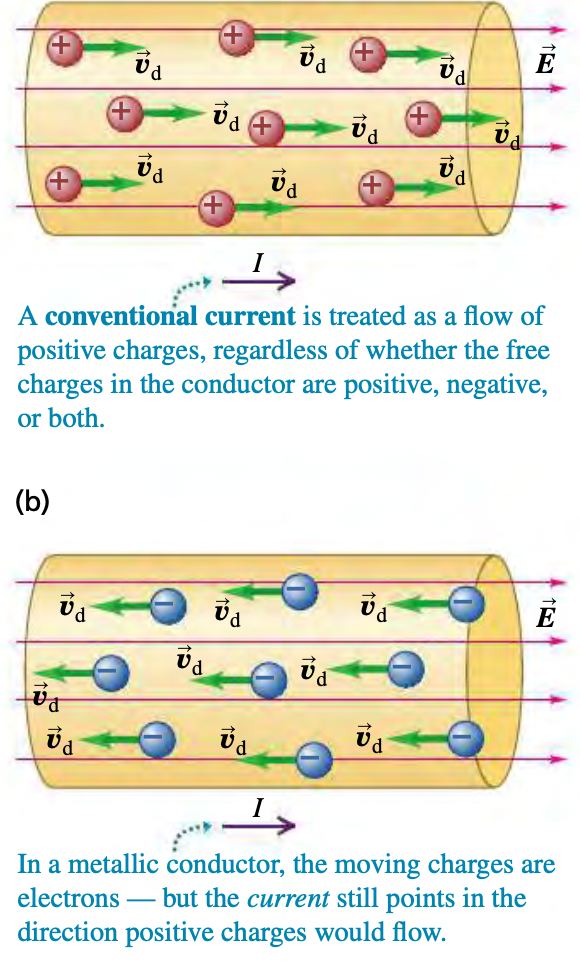
\includegraphics[width=3in]{Media/Current.png}
    \caption{Current Flow Diagram}
    \label{Current Flow Diagram}
\end{figure}


 \begin{definition}
    \textbf{Drift Velocity ($v_d$)}:
    The average velocity of charged particles moving in the direction of the 
    electric force $\vec{F} = q\vec{E}$, though individual charge path is random. 
    This value gives us an alternate calculation of $I$ of 
    $$I = nqv_dA$$ where n is concentration of particles, q is unit charge and A is area.
 \end{definition}

 \subsubsection*{25.1.1 Direction of Current Flow}

\begin{remark}
    Different current-carrying materials may have differently charged moving particles
    In metals the moving charges are always electrons, while in an ionized gas (plasma) or an ionic 
    solution the moving charges may include both electrons and positively charged ions.
    In a semiconductor conduction is partly by electrons and partly by motion 
    of \textit{vacancies}, also known as holes; these are sites of missing electrons 
    and act like positive charges.
\end{remark}

\subsubsection*{25.1.2 Current Density}

\begin{definition}
    \textbf{Current Density (J)}:

   The current per unit cross-section area or $$J = I/A = nqv_d$$ where n is charge concentration, 
   q is the charge per particle and $v_d$ is the drift velocity.
\end{definition}

\subsection*{25.2 Resistivity}

\begin{theorem}
    \underline{Ohm's Law}:
    A relationship in an idealized model that states that the ratio of the electric
    field and the current density is constant in metals at a given temperature, and this is known
    as Resistivity.
\end{theorem}

\begin{definition}
    \textbf{Resistivity ($\rho$)}:
    The permitivity of electrons to move freely in a material, linked with resistance.
    Resistivity is defined as $$ \rho = \frac{E}{J}$$ where E is the magnitude 
    of the electric field and J is the current density. unit is ohm-meters(1 $\Omega \cdot m =V \cdot m/A$)
    Good insulators have high resistivity and conductors have low Resistivity.

    Resistivity can also be calculated as a function of Temperature:
    $$\rho(T) = \rho_0[1+\alpha(T-T_0)]$$ where $\alpha$ is a temperature 
    coefficient of resistivity and  $\rho_0$ being the Resistivity at a reference temperature $T_0$
\end{definition}

\begin{definition}
    \textbf{Conductivity}:
    The recipprocal of resistivity whose units are $(\Omega \cdot m)^{-1}$ Good conductors
    obviously have high Conductivity.
\end{definition}

\begin{definition}
    \textbf{Semiconductor}:
    Materials with propertis intermediate of metals and insulators, whose 
    resistivity is likewise between these two groups.
\end{definition}

\begin{remark}
    A material that obeys Ohm’s law reasonably well is called an \textit{ohmic 
    conductor} or a \textit{linear conductor}, those that dont are \textit{nonohmic}, 
    or \textit{nonlinear}. In the latter materials, J depends on E in a more complicated manner.
\end{remark}

\begin{figure}[H]
    \centering
    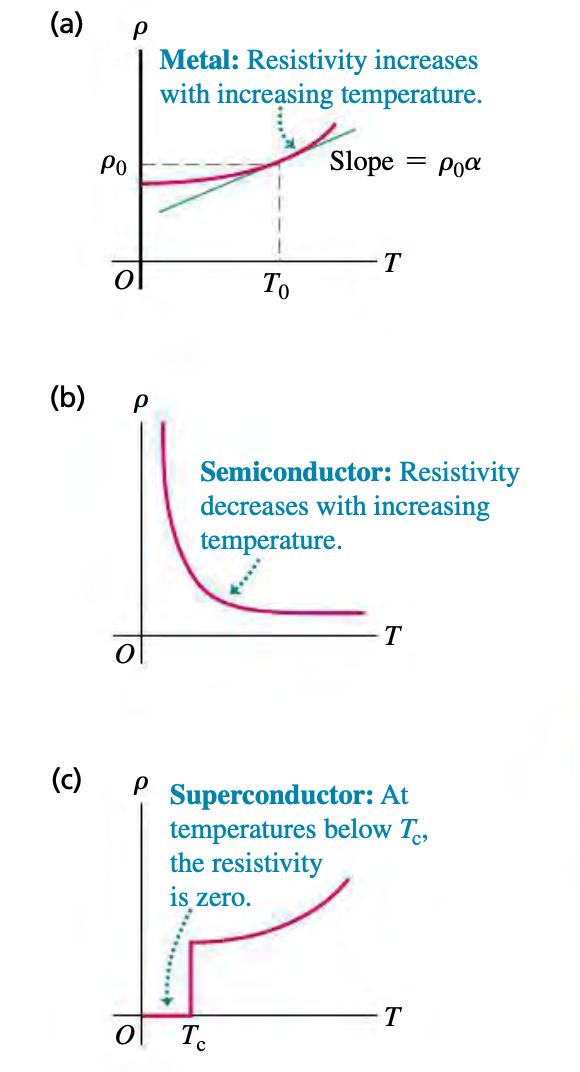
\includegraphics[width=3in,scale=0.25]{Media/Resistivity.png}
    \caption{Resistivity Across Material Types}
    \label{Resistivity Across Material Types}
\end{figure}

\subsection*{25.3 Resistance}

\begin{definition}
    \textbf{Resistance ($R$)}:
    The ratio of Potential Difference V to Current I for a particular conductor.
    Resistance measures the opposition to current flow in an electrical circuit.
    The resistance of a conductor can be calculated by the equation
    $$R = \frac{\rho L}{A} = \frac{V}{I}$$ and its unit is Ohm (1 $\Omega = 1V/A$)
    and similar to resistivity can be a function of Temperature:
    $$R(T) = R_0[1+\alpha(T-T_0)]$$
\end{definition}

\begin{figure}[H]
    \centering
    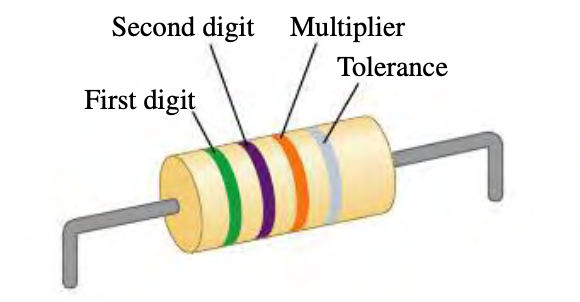
\includegraphics[width=4in]{Media/Resistor.png}
    \caption{Labeling Guide for Resistors}
    \label{Labeling Guide for Resistors}
\end{figure}

\subsection*{25.4 Electromotive Force and Circuits}

\begin{definition}
    \textbf{Electromotive Force ($\mathcal{E}$)}:
    In an electric circuit there must be a device somewhere in the loop that 
    acts like the water pump in a water fountain. This pumping action is called 
    Electromotive Force or emf and the device is called a source of emf. This is not actually
    a force but a energy-per-unit-charge and thus has the unit Volt (1 V = 1 J/C).

    Emf can be calculated in multiple ways:
    $$\mathcal{E} = V_{ab} = IR $$ for ideal sources and where $V_{ab}$ is the Terminal Voltage
    or $$\mathcal{E} = V_{ab} + Ir$$ for when there is internal resistance (r).
\end{definition}

\begin{figure}[H]
    \centering
    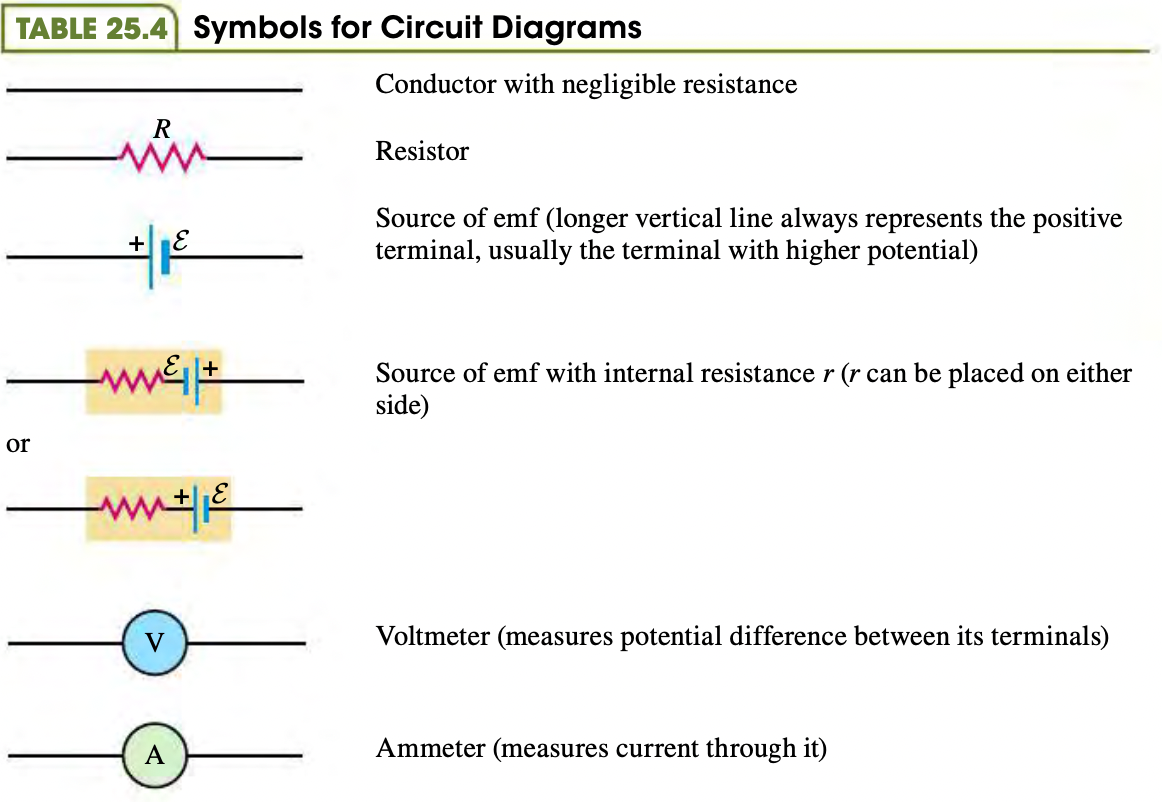
\includegraphics[width=5in]{Media/Circuit.png}
    \caption{Table of Circuit Labels}
    \label{Table of Circuit Labels}
\end{figure}


\subsection*{25.5 Energy and Power in Electric Circuits}

\begin{definition}
    \textbf{Power($P$)}:
    the rate, per unit time, at which electrical energy is transferred in or out of
    an electric element. Power can be found by the following equations:
    $$ P = V_{ab}I = I^2R = \frac{V_{ab}^2}{R} = \mathcal{E}I-I^2r $$
    The SI unit of power is the watt( 1 W = 1 J/s)
    \begin{remark}
        The moving charges in flowing current collide with atoms in the resistor and transfer 
        some of their energy, increasing the \textit{internal energy} of the material. 
        Either the temperature of the resistor increases or there is a flow of heat out of it, or both.  
        Every resistor has a power rating, the maximum power the device can 
        dissipate without becoming overheated and damaged.
    \end{remark}

\end{definition}

\section*{26 Direct-Current Circuits}
Our principal concern in this chapter is with \textit{direct-current (dc}) circuits, 
in which the direction of the current does not change with time. Larger appliances
and household equipment use \textit{alternating current (ac)}, in which the current oscillates back and forth.

\subsection*{26.1 Resistors in Series and Parallel}

\begin{definition}
    \textbf{Series Circuit}:
    When circuit elements are connected in sequence with a single current path 
    between points. In a Series Circuit Capacitors all have the same \textit{Capacitance}
\end{definition}

\begin{definition}
    \textbf{Parallel Circuit}:
    An arrangement where each resistor provides an alternate path between the points. 
    For elements connected in parallel the potential differences is the same across each element.
\end{definition}


\begin{definition}
    \textbf{Equivalent Resistance}:
    The total resistance of a circuit equal to the sum of its parts.
    Equivalent Resistance differes depending on configuration.
    \begin{enumerate}
        \item For Resistors in Series: $R_{eq} = R_1 + R_2 + ..$
        \item For Resistors in Parallel: $\frac{1}{R_{eq}} = \frac{1}{R_1} + \frac{1}{R_2} + ..$
    \end{enumerate}
    \begin{remark}
        The equivalent resistance of a series combination equals the sum of 
        the individual resistances. The equivalent resistance is greater 
        than any individual resistance.The reciprocal of the equivalent 
        resistance of a parallel combination equals the sum of the reciprocals 
        of the individual resistances. The equivalent resistance is always 
        less than any individual resistance.
    \end{remark}
\end{definition}

\subsection*{26.2 Kirschoff's Rules}

\begin{definition}
    \textbf{Junction}:
    A junction in a circuit is a point where three or more conductors meet.
\end{definition}

\begin{definition}
    \textbf{Loop}:
    A loop is any closed conducting path in a circuit, including the circuit itself.
\end{definition}

\begin{figure}[H]
    \centering
    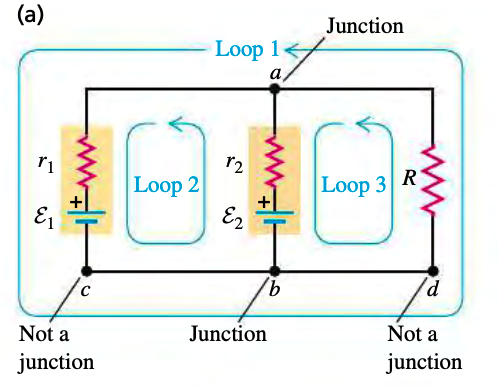
\includegraphics[width=3in,scale=0.25]{Media/Junctionloop.png}
    \caption{Example of Junctions and Loops}
    \label{Example of Junctions and Loops}
\end{figure}

\begin{definition}
    \textbf{Kirschoff's Junction Rule}:
    The sum of the currents into any junction is 0, or in other words the current
    that flows in a junction must equal the current flowing out the junction.
    $$\Sigma I =0$$
    This is valid at any junction.
\end{definition}

\begin{definition}
    \textbf{Kirschoff's Loop Rule}:
    The sum of the potential differences around any loop must equal 0, or in other 
    words the sum voltage at the end of a circuit or loop must equal 0.
    $$\Sigma V =0$$
    This is valid at any closed loop.
\end{definition}

\begin{figure}[H]
    \centering
    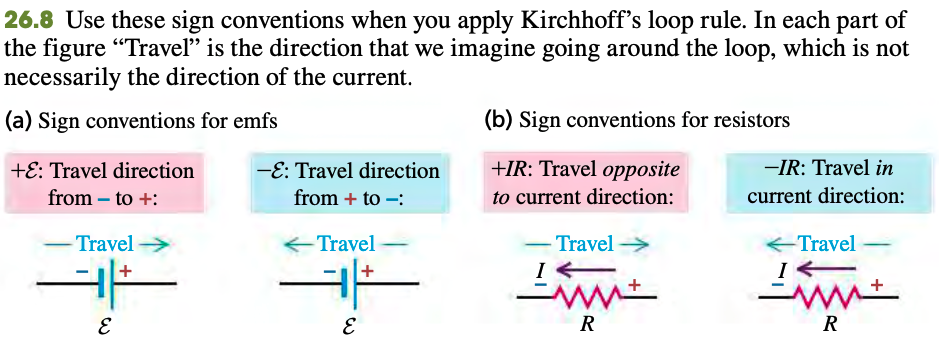
\includegraphics[width=5in,scale=0.25]{Media/Loopsign.png}
    \caption{Picking a sign for loops}
    \label{Picking a sign for loops}
\end{figure}

\subsection*{26.3 Electrical Measuring Instruments}

\begin{definition}
    \textbf{d’Arsonval galvanometer}:
    Tool used to measure potential difference, current, or resistance by evaluating
    the torque caused by the magnetic field on a coil by current.For a larger 
    current range, a shunt resistor is added, so some of the current bypasses the meter coil, 
    and this makes an ammeter. If materials are ohmic the ammeter can be converted toa voltmeter
\end{definition}

\begin{remark}
    Ammeters should be placed in series with resistors to measure current due to 
    having little resistance and thus drawing current. Voltmeters should be attatched
    in parallel as they have very high resistance and thus can block current Flow
    if attatched in series.
\end{remark}

\begin{figure}[H]
    \centering
    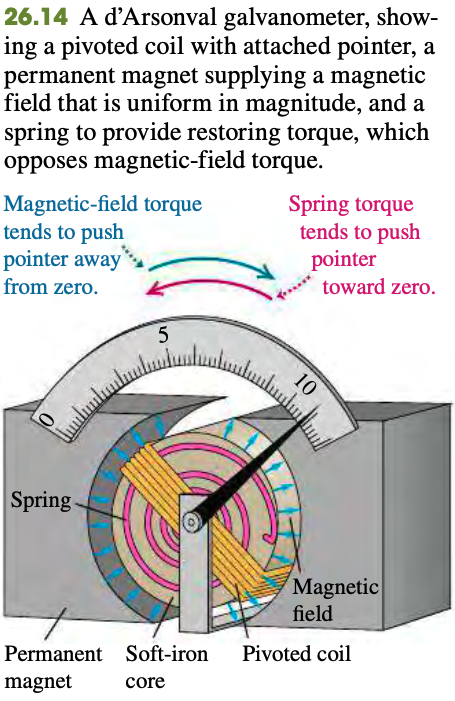
\includegraphics[width=3in,scale=0.25]{Media/galvano.png}
    \caption{Example of d’Arsonval galvanometer}
    \label{Example of d’Arsonval galvanometer}
\end{figure}


\subsection*{26.4 R-C Circuits}

\begin{definition}
    \textbf{R-C Circuit}:
    A circuit containing resistors and capacitors in series with an ideal battery
    and ideal wires. In these circuits we take into consideration time to charge 
    a capacitor, as time is not constant. For these situations use the following
    equations:
    \begin{enumerate}
        \item For Charge: $$q = C\mathcal{E}(1-e^{-t/RC}) = Q_f(1-e^{-t/RC})$$
        Where $t$ is time since switch closed and $Q_f$ is final capacitor charge =$C\mathcal{E}$
        \item For Current: $$i = \frac{dq}{dt} = \frac{\mathcal{E}}{R}e^{-t/RC} = I_0e^{-t/RC}$$
        Where $t$ is time since switch closed and $I_0$ is initial current charge =$\mathcal{E}/R$
        \begin{remark}
            Variables are in lower case to distinguish they are time-varying quantities
            and seperate from their constant capitalized counterparts.
        \end{remark}
    \end{enumerate}
\end{definition}

\begin{figure}[H]
    \centering
    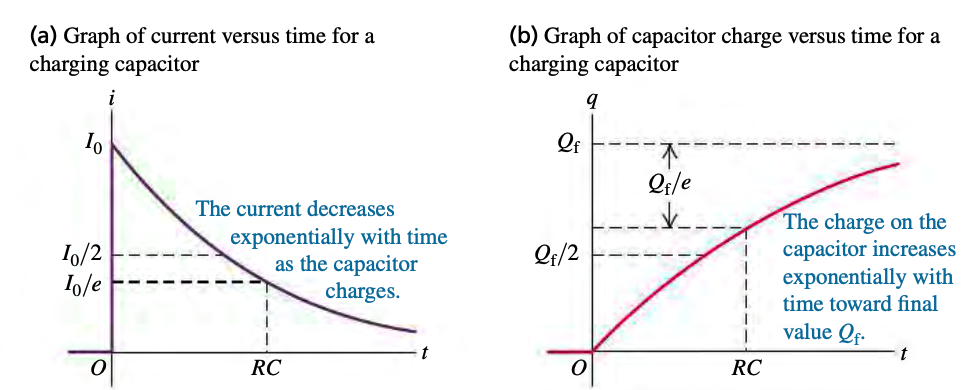
\includegraphics[width=5in]{Media/Charging.png}
    \caption{Capacitor Charging Curve}
    \label{Capacitor Chargeing Curve}
\end{figure}

\subsubsection*{26.4.1 Time Constant}

\begin{definition}
    \textbf{Time Constant ($\tau$)}:
    A time constant is the time equal to RC or the time at which the current has decreased
    to 1/e its original value and the capacitor has reached (1-1/e) its final value $Q_f = C\mathcal{E}$
    It is thus a measure of how quickly a capacitor charges. It can be calculated with $$\tau = RC$$
    The unit for $\tau$ is seconds ($1 s = 1 F \cdot C$)
    \begin{remark}
        When $\tau$ is small, the capacitor charges quickly; 
        when it is larger, the charging takes more time.
    \end{remark}

\end{definition}

\subsubsection*{26.4.2 Discharging a Capacitor}

\begin{remark}
    The functions for discharging a Capacitor are the same as for charging except
    that the sign of current is opposite as current is flowing out
    \item For Charge: $$q = Q_f(1-e^{-t/RC})$$
        Where $t$ is time since switch closed and $Q_f$ is initial capacitor charge =$C\mathcal{E}$
        \item For Current: $$i = \frac{dq}{dt} = -\frac{{Q_0}}{RC}e^{-t/RC} = I_0e^{-t/RC}$$
        Where $t$ is time since switch closed and $I_0$ is initial current charge =$-Q_0/RC$
\end{remark}

\begin{figure}[h]
    \centering
    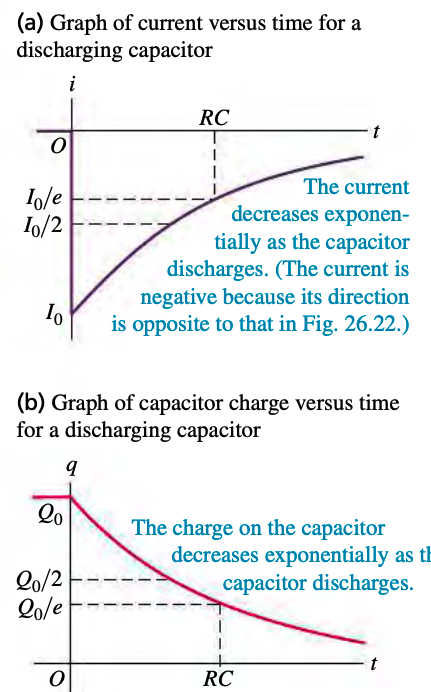
\includegraphics[width=3in,scale=0.25]{Media/Discharging.png}
    \caption{Capacitor Discharging Curve}
    \label{Capacitor Discharging Curve}
\end{figure}

\end{document}